\documentclass[11pt]{article}

\usepackage[a4paper, margin=1in]{geometry}
\usepackage{amsmath}
\usepackage{amssymb}
\usepackage{graphicx}
\graphicspath{{figures/numpy_exact/}}
\usepackage{placeins}
\usepackage[hidelinks]{hyperref}

\newcommand{\ket}[1]{\left|#1\right\rangle}
\newcommand{\ev}[1]{\left\langle #1 \right\rangle}
\setlength{\parindent}{0pt}

\title{Learning Notes: Two-Qubit Hamiltonian Simulation}
\author{QClp-Qiskit Project}

\begin{document}

\maketitle

\begin{abstract}
These notes summarize the learning process behind a two-qubit Hamiltonian
simulation project. The project compares a direct NumPy/SciPy exact
statevector simulation with a Qiskit circuit-based statevector simulation.
The focus is on understanding the model, the role of each Hamiltonian term,
the meaning of the observables, and the numerical checks used to validate the
two implementations.
\end{abstract}

\section{Project Content}

This project focuses on a small two-qubit Hamiltonian simulation. The main
content includes:
\begin{itemize}
  \item Time evolution for a two-qubit quantum system based on Hamiltonian.
  \item Statevector representation of the four basis states.
  \item Exact matrix-exponential simulation with NumPy/SciPy.
  \item Expectation-value calculation and observation.
  \item Statevector circuit simulation with Qiskit.
  \item Comparison between the matrix-based reference result and the Qiskit circuit representation.
\end{itemize}
With only two qubits, the statevector has four components and the Hamiltonian
is a $4 \times 4$ matrix. This makes the system suitable for direct learning,
debugging, and numerical verification.


\vspace{\baselineskip}


\section{Two-Qubit State Representation}
\subsection{Computational Basis}
The single-qubit basis states are $\ket{0}$ and $\ket{1}$. For two qubits, the  basis are
\begin{align*}
  \ket{00} \, ,\quad \ket{01} \, ,\quad \ket{10} \, ,\quad \ket{11} \, .
\end{align*}
a general two-qubit state can be written as
\begin{align*}
    \ket{\psi} = a\ket{00} + b\ket{01} + c\ket{10} + d\ket{11} \, , \quad
    \text{where }\, a \, , b \, , c \, , d \,\in \mathbb{C}
\end{align*}
and the squared norms of these amplitudes $|a|^2$, $|b|^2$, $|c|^2$, and $|d|^2$ stand for the probabilities of measuring the corresponding basis states.\\

In two-qubit system, $\ket{00}$ and $\ket{11}$ have two qubits in the same direction, these two basis states are called \textbf{aligned states}, while $\ket{01}$ and $\ket{10}$ are called \textbf{anti-aligned states} for they have two qubits in the different direction.

\vspace{\baselineskip}

\subsection{Tensor-Product Operators}
For two-qubit system, single-qubit operators are extended to the four-dimensional state space using tensor products. 

Let $X$ and $Z$ be Pauli matrices in single-qubit system, and let $I$ be the identity operator, then we have:
\begin{gather*}
    Z_0 = Z \otimes I \, , \qquad
    Z_1 = I \otimes Z \, , \qquad
    Z_0Z_1 = Z \otimes Z \, .\\
    X_0 = X \otimes I \, , \qquad
    X_1 = I \otimes X \, . 
\end{gather*}


\vspace{\baselineskip}


\section{Hamiltonian Model}
In this project, the Hamiltonian is
\begin{align*}
  H = J Z_0 Z_1 + h(X_0 + X_1),
\end{align*}
with parameters
\begin{align*}
  J = 1.0,\qquad h = 0.5.
\end{align*}
The project studies the four initial states
\begin{align*}
  \ket{00} \, , \quad \ket{01} \, , \quad \ket{10} \, , \quad \ket{11} \, ,
\end{align*}
on the time grid \texttt{np.linspace(0, 10, 200)}.

Denote $H_Z := J Z_0 Z_1$ and  $H_X := h(X_0 + X_1)$\,, then $H = H_Z + H_X$.

\vspace{\baselineskip}

\subsection{Role of the $H_Z$ Term}
For a single-qubit system, the $Z$ gate (operator) distinguishes the qubit's orientation in the Z-basis:
\begin{align*}
  Z\ket{0} = +\ket{0} \, ,\qquad Z\ket{1} = -\ket{1} \, ,
\end{align*}
so the $Z_0Z_1$ term defines the aligned and anti-aligned structure in the
$Z$ basis:
\begin{align*}
  Z_0Z_1\ket{00} &= +\ket{00} \, , &
  Z_0Z_1\ket{11} &= +\ket{11} \, , \\
  Z_0Z_1\ket{01} &= -\ket{01} \, , &
  Z_0Z_1\ket{10} &= -\ket{10} \, .
\end{align*}
It's clear that for aligned states $\ket{00}$ and $\ket{11}$\,, $Z_0Z_1$ assigns them the eigenvalue $+1$\,, while for anti-aligned states $\ket{01}$ and $\ket{10}$\,, $Z_0Z_1$ assigns them $-1$\,. 
The results imply that the operator $Z_0Z_1$ detects whether the two qubits are aligned or anti-aligned, thereby turning two independent qubits into an interacting two-qubit spin system.
In this sense, $Z_0Z_1$ can be understood as a $Z$-direction correlation operator.

\vspace{\baselineskip}

\subsection{Role of the $H_X$ Term}
For a single-qubit system, the $X$ gate (operator) swaps the $\ket{0}$ and $\ket{1}$ states:
\begin{align*}
  X\ket{0} = \ket{1} \, , \quad
  X\ket{1} = \ket{0} \, .
\end{align*}
So the $X_0 + X_1$ term drives amplitude flow among four basis states
by flipping one qubit at a time. More precisely, for the initial state $\ket{00}$:
\begin{gather*}
  X_0\ket{00} = \ket{10} \, , \: \: X_1\ket{00} = \ket{01} \, , \\
  (X_0 + X_1)\ket{00} = \ket{10} + \ket{01} \, .
\end{gather*}
and for other basis states:
\begin{align*}
    (X_0 + X_1)\ket{01} = \ket{11} + \ket{00} \, , \\
    (X_0 + X_1)\ket{10} = \ket{00} + \ket{11} \, , \\
    (X_0 + X_1)\ket{11} = \ket{01} + \ket{10} \, .
\end{align*}
This means that for an arbitrary statevector in a two-qubit system
\begin{align*}
    \ket{\psi} = a\ket{00} + b\ket{01} + c\ket{10} + d\ket{11} \, ,
\end{align*}
the amplitudes of $\ket{00}$ and $\ket{11}$ can flow
into the directions in $\ket{10}$ and $\ket{01}$, and the amplitudes of $\ket{01}$ and $\ket{10}$ will flow to directions $\ket{00}$ and $\ket{11}$ during time evolution. In this way, the $H_X$ term drives the initial amplitudes of the statevector to transfer and circulate among the basis-state directions $\ket{00}, \ket{01}, \ket{10}, \ket{11}$ during time evolution.\\

In conclusion, the role of $H_X$ is to couple the four basis states by flipping a single qubit, causing the complex amplitudes to circulate and oscillate among these basis-state directions during time evolution.


\vspace{\baselineskip}


\section{Simulation Methods}

\subsection{NumPy/SciPy Exact Simulation}
The NumPy implementation is the reference calculation. It directly constructs
the Pauli matrices, tensor-product operators, Hamiltonian matrix, and
time-evolution operator. The core calculation is
\begin{align*}
  U(t) = e^{-iHt} \, , \qquad  \ket{\psi(t)} = U(t)\ket{\psi(0)} \, .
\end{align*}
This method is direct and reliable for a two-qubit system because the
Hamiltonian is only a $4 \times 4$ matrix.

\vspace{\baselineskip}

\subsection{Qiskit Statevector Simulation}
The Qiskit implementation is used to reproduce the same statevector dynamics in a circuit representation. It represents the same Hamiltonian dynamics in circuit
form. It uses
\begin{itemize}
  \item \texttt{SparsePauliOp} to define the Hamiltonian and observables,
  \item \texttt{PauliEvolutionGate} to express time evolution as a circuit
        operation,
  \item \texttt{Statevector} to simulate the resulting circuit state.
\end{itemize}
The Qiskit implementation was reviewed against the NumPy reference and the intended project scope.


\vspace{\baselineskip}


\section{Observables and Interpretation}

The project calculates three observables:
\begin{itemize}
  \item $\ev{Z_0}(t)$: the $Z$-direction expectation value of the first qubit, measuring whether the first qubit is biased toward $\ket{0}$ or $\ket{1}$ , 
  \item $\ev{Z_1}(t)$: the $Z$-direction expectation value of the second qubit, measuring whether the second qubit is biased toward $\ket{0}$ or $\ket{1}$ , 
  \item $\ev{Z_0Z_1}(t)$: a two-qubit correlation observable, measuring whether the two qubits are biased toward being aligned or anti-aligned.
\end{itemize}
These observables make the state evolution easier to interpret. Instead of
only inspecting the full statevector, the plots show how measurable quantities
change over time.

\begin{figure}[htbp]
  \centering
  \begin{minipage}{0.48\textwidth}
    \centering
    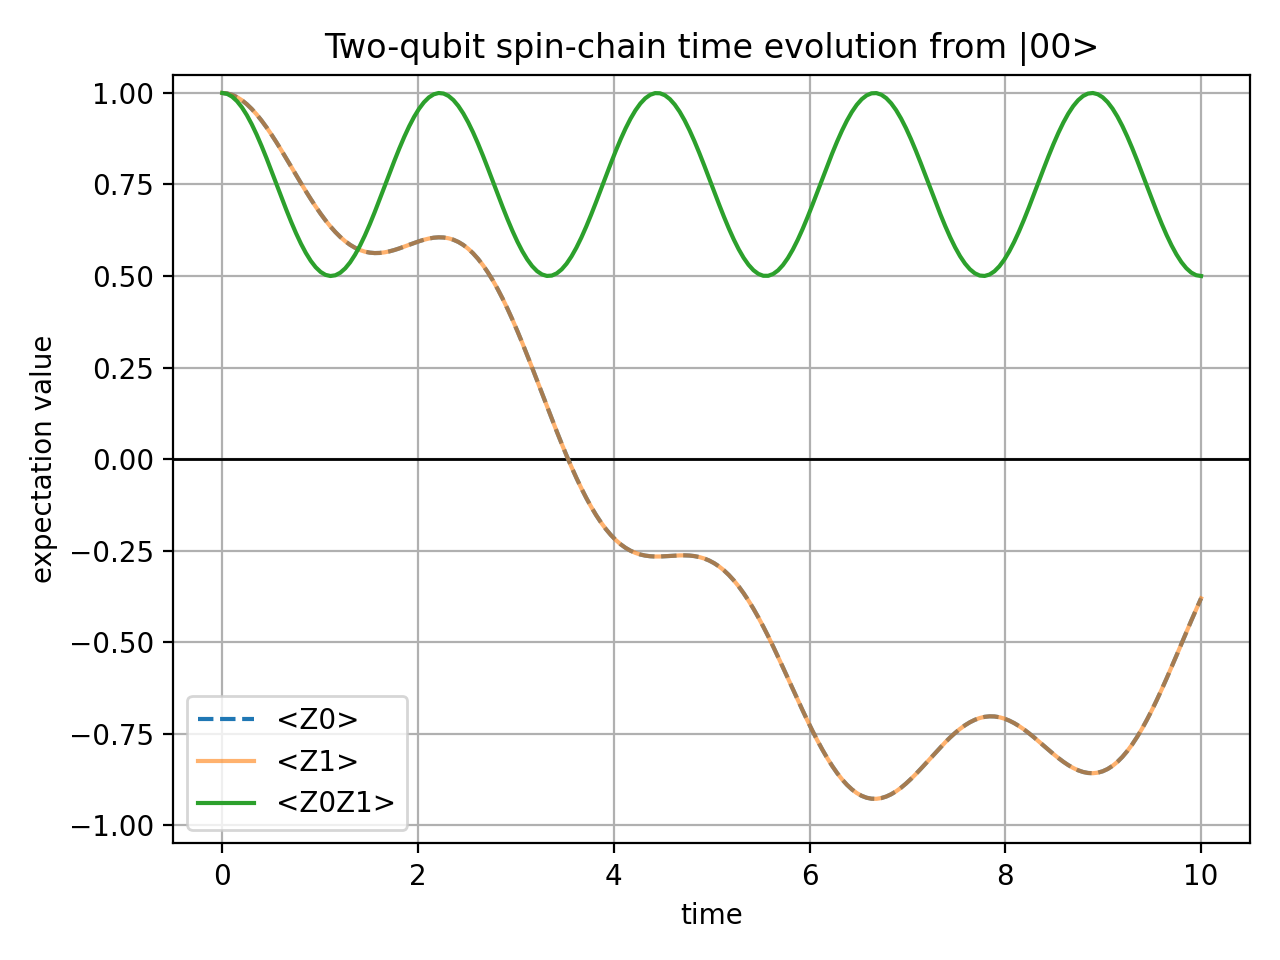
\includegraphics[width=\linewidth]{Initial_00_expvl.png}
    \vspace{0.3em}
    {\small Initial state $\ket{00}$}
  \end{minipage}
  \hfill
  \begin{minipage}{0.48\textwidth}
    \centering
    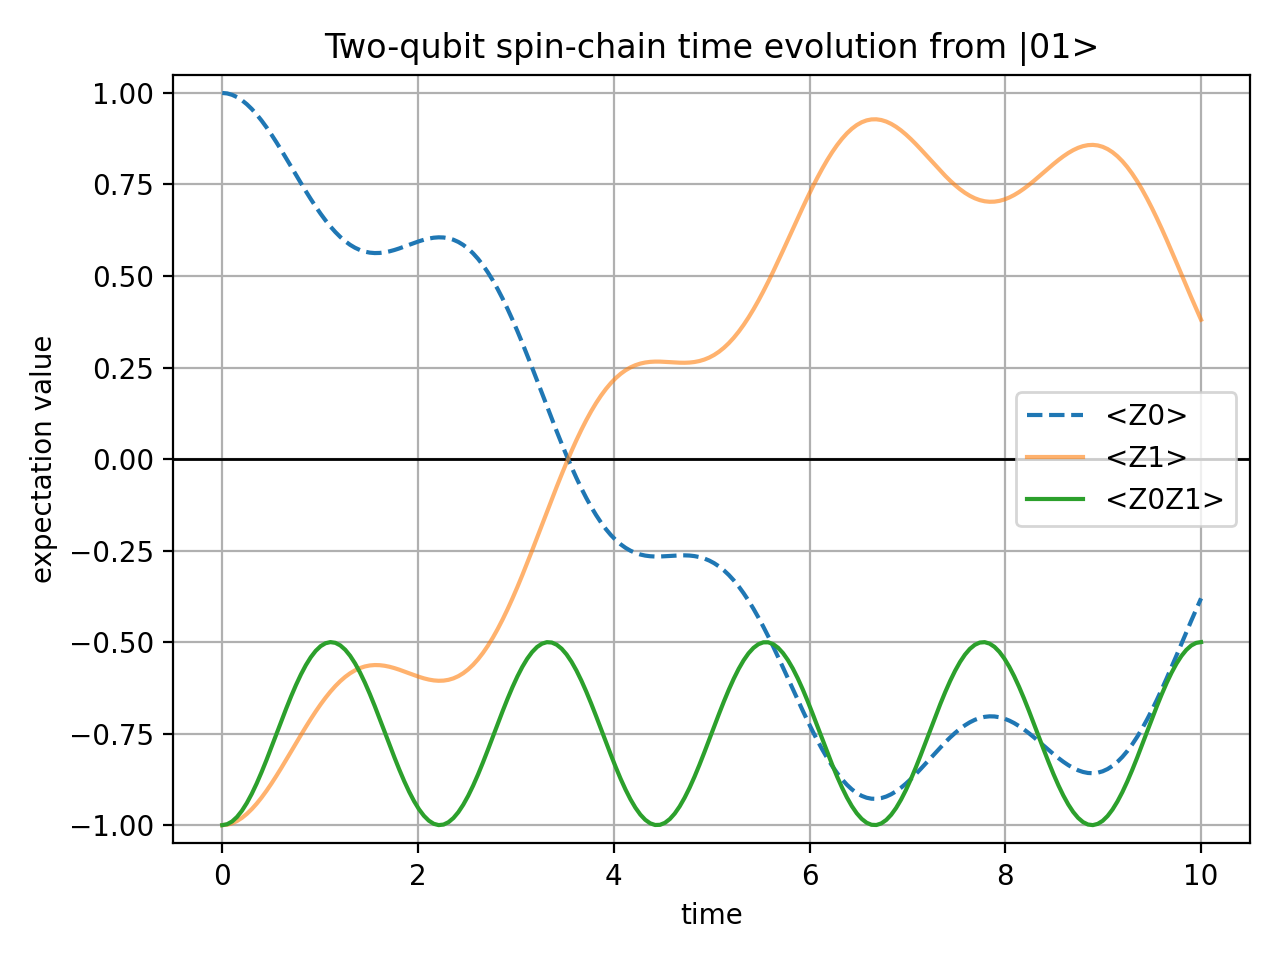
\includegraphics[width=\linewidth]{Initial_01_expvl.png}
    \vspace{0.3em}
    {\small Initial state $\ket{01}$}
  \end{minipage}
  \caption{Expectation-value curves for initial states $\ket{00}$ and $\ket{01}$ from the NumPy exact simulation.}
  \label{fig:numpy-initial-00-01}
\end{figure}

\begin{figure}[htbp]
  \centering
  \begin{minipage}{0.48\textwidth}
    \centering
    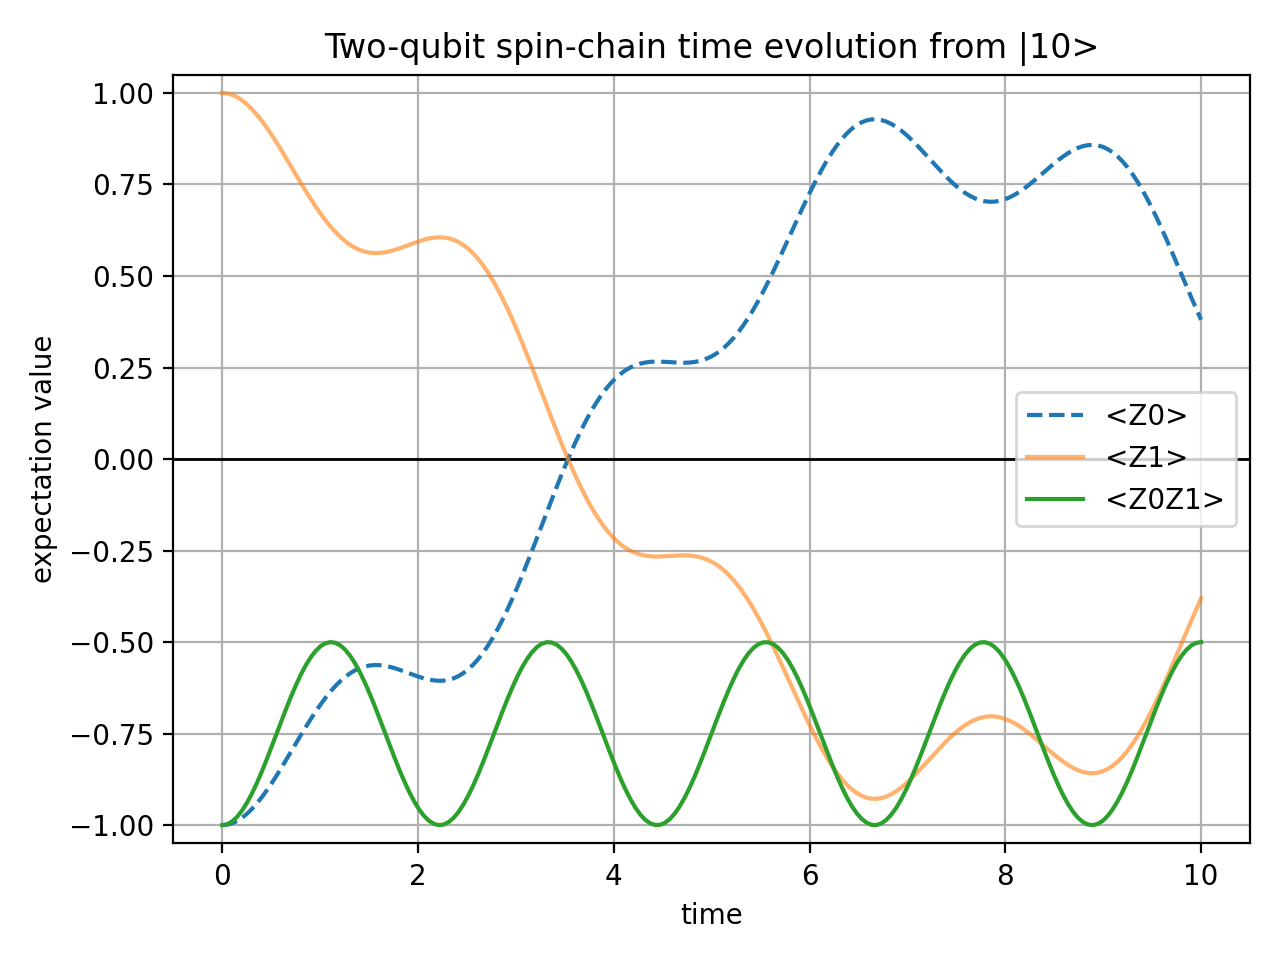
\includegraphics[width=\linewidth]{Initial_10_expvl.png}
    \vspace{0.3em}
    {\small Initial state $\ket{10}$}
  \end{minipage}
  \hfill
  \begin{minipage}{0.48\textwidth}
    \centering
    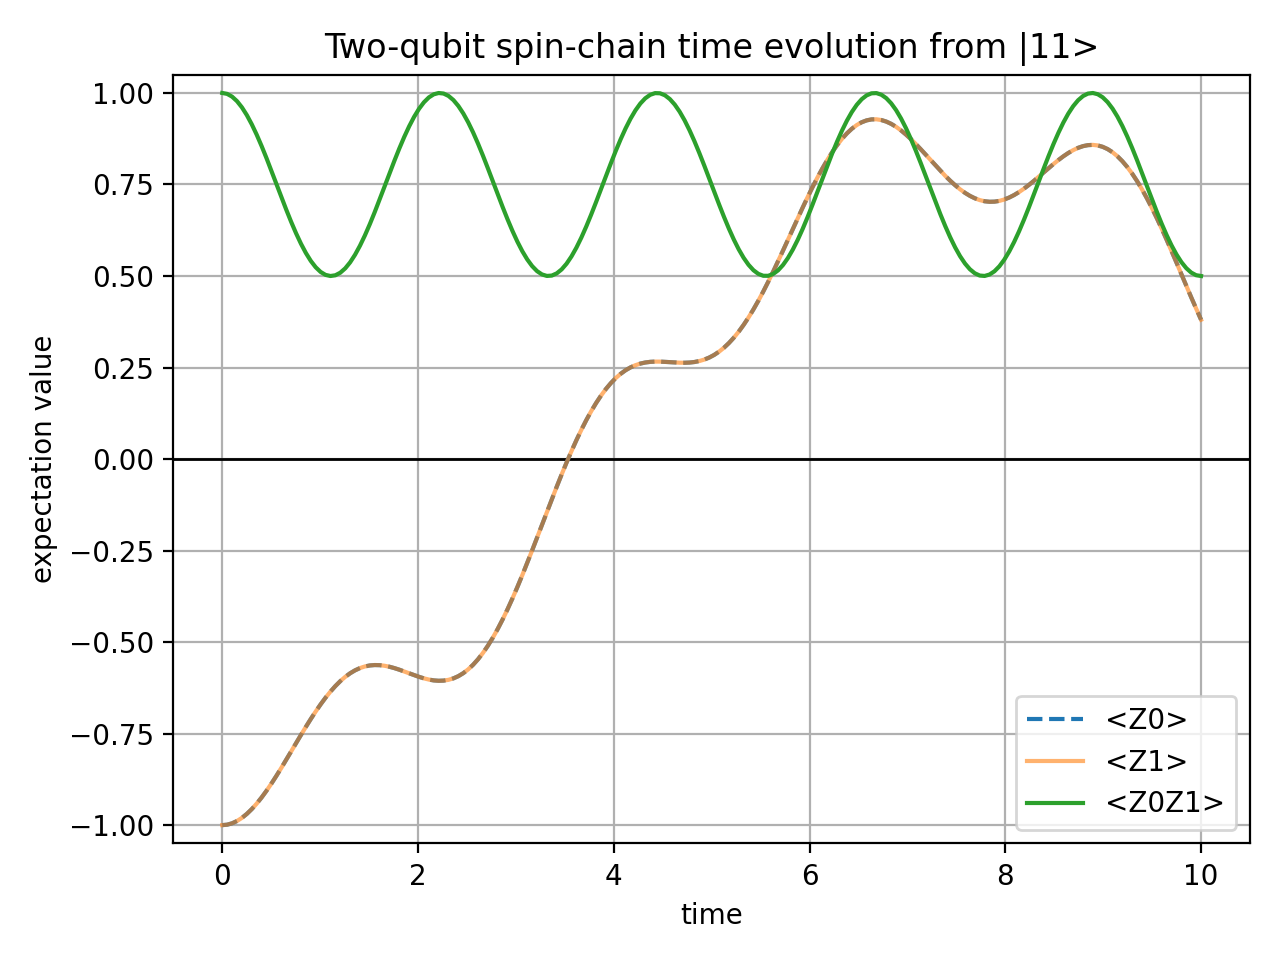
\includegraphics[width=\linewidth]{Initial_11_expvl.png}
    \vspace{0.3em}
    {\small Initial state $\ket{11}$}
  \end{minipage}
  \caption{Expectation-value curves for initial states $\ket{10}$ and $\ket{11}$ from the NumPy exact simulation.}
  \label{fig:numpy-initial-10-11}
\end{figure}

\FloatBarrier

Figures~\ref{fig:numpy-initial-00-01} and~\ref{fig:numpy-initial-10-11} show
how the same Hamiltonian produces different expectation-value curves from
different initial basis states.

If a general two-qubit state is written as
\begin{align*}
  \ket{\psi}
  = a\ket{00} + b\ket{01} + c\ket{10} + d\ket{11} \, ,
\end{align*}
then the three observables can be interpreted through the probability weights
of the basis-state components. The expectation value $\ev{Z_0}$ compares
the total probability weight of states where the first qubit is $\ket{0}$ with
those where it is $\ket{1}$:
\begin{align*}
  \ev{Z_0} = |a|^2 + |b|^2 - |c|^2 - |d|^2.
\end{align*}
Similarly, $\ev{Z_1}$ compares the corresponding weights for the second
qubit:
\begin{align*}
  \ev{Z_1} = |a|^2 - |b|^2 + |c|^2 - |d|^2.
\end{align*}
The correlation observable $\ev{Z_0Z_1}$ compares the aligned components
$\ket{00}$ and $\ket{11}$ with the anti-aligned components $\ket{01}$ and
$\ket{10}$:
\begin{align*}
  \ev{Z_0Z_1} = |a|^2 - |b|^2 - |c|^2 + |d|^2.
\end{align*}

The initial value of $\ev{Z_0Z_1}$ separates aligned and anti-aligned
states:

\begin{itemize}
  \item $\ket{00}$ and $\ket{11}$ start with $\ev{Z_0Z_1}=+1$,
  \item $\ket{01}$ and $\ket{10}$ start with $\ev{Z_0Z_1}=-1$.
\end{itemize}

The model is symmetric under exchanging qubit 0 and qubit 1. This symmetry
explains why $\ket{01}$ and $\ket{10}$ produce related curves with
$\ev{Z_0}$ and $\ev{Z_1}$ interchanged.\\

During time evolution, the transverse-field term $H_X$ drives the amplitudes to circulate among different basis-state directions, which in turn causes the expectation values involving Z to oscillate. For this reason, the plotted curves therefore show both the interaction structure defined by $Z_0Z_1$ and the effect of the transverse field $X_0 + X_1$.\\

In this way, the plots show how the evolving amplitudes appear through physically interpretable $Z$-basis
observables.


\vspace{\baselineskip}


\section{Scope and Possible Extensions}
The completed scope is:
\begin{center}
  NumPy exact result $\rightarrow$ Qiskit statevector result $\rightarrow$
  numerical comparison $\rightarrow$ plots
\end{center}
The completed version intentionally does not include Qiskit Aer backends,
noise models, shot-based execution, real hardware execution, or Trotter error
analysis.

Possible local extensions include:
\begin{itemize}
  \item Trotter error analysis for comparing exact evolution with
        product-formula approximations,
  \item parameter sweeps over different $J$, $h$, and total evolution time,
  \item extension from two qubits to small spin chains,
  \item additional observables, such as entanglement entropy or state fidelity.
\end{itemize}


\vspace{\baselineskip}


\section{Summary}

This project shows a complete learning path from a simple Hamiltonian model to
two working simulations and numerical validation. The NumPy implementation
provides the exact reference result, while the Qiskit implementation reproduces
the same dynamics through statevector circuit simulation.

\end{document}
